\section{Characterizing Residual Idle Capacity in \ac{MoE} Serving}
\label{sec:characterization}

\mv{This is a study in itself, very in-depth!}

\acresetall

Load imbalance and the resulting stragglers in expert-parallel \ac{MoE}
execution are well known (\S\ref{sec:bg-moe}). Our goal is not to
establish their existence, but to determine whether the idle intervals
they leave behind constitute a useful and schedulable source of GPU
capacity.

We answer five questions. First, \emph{where} during inference does routing
imbalance translate into a harvestable bubble? Second, once such bubbles
arise, how large are they and how does their size scale with the amount of
prefill work? Third, do modern serving optimizations---including expert
load balancing and lower-precision execution---eliminate this opportunity,
or does useful slack remain? Fourth, how does bubble size vary across
models, workloads, hardware, and parallelism configurations? Finally,
despite this variation, can the available slack be predicted early enough
to safely schedule work into it? Together, these measurements characterize
the resource that \sys{} targets and derive the requirements its scheduler
must satisfy.

\label{sec:char-method}
\paragraph{Bubble definition.}
Figure~\ref{fig:anatomy} illustrates where residual idle time arises in an
expert-parallel \ac{MoE} layer. After routing and dispatch, each rank
executes the experts assigned to its local tokens. Because routing is
input-dependent, ranks may receive different amounts of expert work and
therefore finish their local \ac{GEMM}s at different times.
\mv{Maybe this should go to the background already}

For rank $r$ in layer $\ell$, we define a \emph{bubble} as the interval
between $r$ completing its local expert computation and the cross-rank
combine being able to proceed. In Figure~\ref{fig:anatomy}, Rank~0 receives
less expert work and finishes before Rank~1; Rank~0 therefore remains idle
until Rank~1 reaches the combine. This waiting interval is Rank~0's bubble.
It is residual rank-local capacity that a colocated workload can reclaim,
provided that the admitted work completes before the synchronization
dependency clears.

\begin{figure}[t]
  \centering
  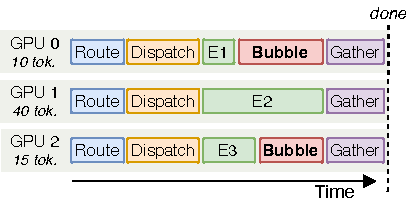
\includegraphics[width=0.82\linewidth]{figures/bubble.drawio.pdf}
  \caption{
    \textbf{Definition of an expert-parallel bubble.}
    Top: an \ac{MoE} layer routes tokens to their top-$k$ experts,
    dispatches them across ranks, executes grouped expert \ac{GEMM}s,
    and combines the resulting expert outputs.
    Bottom: input-dependent routing assigns fewer tokens to Rank~0
    than Rank~1. Rank~0 consequently finishes its local expert
    computation first but cannot proceed until the more heavily loaded
    Rank~1 reaches the combine. We define this rank-local waiting
    interval as Rank~0's \emph{bubble}.
  }
  \Description{
    The top panel shows the execution stages of an expert-parallel MoE
    layer: routing, dispatch, expert computation, combine, and output.
    The bottom panel compares two GPU ranks. Rank 0 receives fewer
    tokens and finishes expert computation before Rank 1. Rank 0 then
    remains idle until Rank 1 finishes and the combine can proceed.
    This waiting interval is labeled the bubble.
  }
  \label{fig:anatomy}
\end{figure}

\paragraph{Measurement.}
We instrument \ac{MoE} execution with CUDA events and measure, for each
rank and layer, the interval between completion of its local expert
computation and the synchronization that allows the layer to proceed.
In our vLLM execution path, the measurement window terminates at the
tensor-parallel all-reduce. Consequently, these measurements capture the
rank-local idle interval defined above and should not be interpreted as
DeepEP dispatch/combine latency.

\OPEN{If the SGLang/LPLB/Waterfill experiments use a different execution
  path or measurement boundary, report them separately rather than combining
them with the vLLM measurements.}

\paragraph{Experimental setup.}
Unless stated otherwise, experiments use two NVIDIA A100 80,GB GPUs with
\ac{TP}$=2$ for the non-expert parameters and \ac{EP}$=2$ for expert parameters,
the Triton grouped-\ac{GEMM} \ac{MoE} backend, and an allgather/reduce-scatter
all-to-all implementation. We evaluate the three models in Table~\ref{tab}.
Inputs are real arxiv-summarization prompts truncated to the
requested context length,
and we report medians across repetitions unless stated otherwise.
\S\ref{sec:char-method} uses the same default setup.

\begin{table}[t]
  \centering
  \small
  \caption{Models used throughout \S\ref{sec:characterization}.}
  \label{tab}
  \begin{tabular}{lrll}
    \toprule
    Model & \ac{MoE} layers & Experts & Routing \\
    \midrule
    Qwen3-30B-A3B & 48 & 128 & top-8 \\
    Qwen1.5-MoE-A2.7B & 24 & 60 + 4 shared & top-4 \\
    DeepSeek-V2-Lite & 27 & 64 + 2 shared & top-6 \\
    \bottomrule
  \end{tabular}
\end{table}

\subsection{Bubbles arise primarily during prefill}
\label{sec:char-phase}

Routing imbalance alone does not determine whether useful idle capacity
appears: the imbalance must be large enough in absolute execution time to
create a harvestable interval. We therefore compare prefill and decode
using both \emph{routing skew} and the resulting rank-to-rank
expert-compute gap. We define routing skew as the maximum routed-token
count across ranks divided by the mean, so that larger values indicate
greater imbalance.\footnote{This is the inverse of vLLM's
\emph{balancedness} statistic.} We measure the rank \ac{GEMM} gap per
layer, as the difference between the two ranks' total expert-\ac{GEMM}
time within that layer, from matched profiler traces. Load balancing is
disabled throughout.

\begin{table}[t]
  \centering
  \small
  \caption{
    \textbf{Decode is more imbalanced in relative terms, but only prefill
    produces millisecond-scale rank-time differences.}
    Qwen3-30B-A3B, \ac{TP}$=2$, \ac{EP}$=2$, with load balancing disabled.
    \ac{GEMM} gaps are per \ac{MoE} layer.
  }
  \label{tab:phase}
  \begin{tabular}{lcc}
    \toprule
    & Prefill & Decode \\
    \midrule
    Routing skew (arxiv) & 1.28$\times$ & 1.75$\times$ \\
    Routing skew (MMLU)  & 1.26$\times$ & 1.63$\times$ \\
    \midrule
    Workload size
    & 8k--128k tokens
    & batch 1--128 \\
    Rank \ac{GEMM} gap, p50
    & 0.29--6.80\,ms
    & 0\,$\mu$s \\
    Rank \ac{GEMM} gap, p90
    & 0.89--17.6\,ms
    & 14--42\,$\mu$s \\
    \bottomrule
  \end{tabular}
\end{table}

Table~\ref{tab:phase} reveals an apparent paradox. Decode has greater
relative routing skew: its max-to-mean ratio reaches
$1.75\times$ on arxiv and $1.63\times$ on MMLU, compared with
$1.28\times$ and $1.26\times$ during prefill. A decode step routes
relatively few tokens, making its realized expert distribution noisier.
Yet the resulting rank-to-rank expert-\ac{GEMM} gap stays in the
microseconds across decode batch sizes from 1 to 128: its median is
0\,$\mu$s/layer and even its p90 is at most 42\,$\mu$s/layer. During
prefill, in contrast, the median gap grows from 0.29\,ms/layer at 8k
tokens to 6.80\,ms/layer at 128k, in line with the bubbles measured
directly in \S\ref{sec:char-context}  (6.41\,ms/layer at 128k).

Thus, the resource \sys{} harvests is not routing imbalance itself, but
the \emph{absolute timing difference} that imbalance creates between
ranks. Prefill executes substantially more expert work per layer, turning
even smaller relative skew into millisecond-scale rank stalls, whereas
decode's larger relative skew produces negligible rank-local waiting.
\sys{} therefore targets expert-parallel bubbles primarily during
prefill.

\takeaway{1}{
  Routing imbalance occurs in both phases and is larger during decode, but
  harvestable bubbles arise primarily during prefill, where routing skew
  becomes millisecond-scale rank-to-rank execution-time differences.
}
\subsection{Bubbles grow with prefill size}
\label{sec:char-context}

\begin{figure}[t]
  \centering
  \inputplot{context_bubble}
  \caption{
    \textbf{Bubble size grows substantially with prefill size.}
    Median per-layer bubble across three \ac{MoE} architectures under BF16
    execution without load balancing. Error bars show min/max across
    repetitions.
  }
  \label{fig:context}
\end{figure}

Figure~\ref{fig:context} shows that longer prefills expose substantially
larger rank-local idle intervals across all three \ac{MoE} architectures.
At 128k tokens, the median bubble reaches 6.41\,ms/layer on
Qwen3-30B-A3B, 4.34\,ms/layer on Qwen1.5-MoE-A2.7B, and
2.70\,ms/layer on DeepSeek-V2-Lite.

These intervals recur at every \ac{MoE} layer rather than forming one
continuous idle period. At 128k, the median per-layer bubbles correspond
to approximately 308\,ms, 104\,ms, and 73\,ms of cumulative rank-local
idle time over one forward pass on Qwen3, Qwen1.5-MoE, and
DeepSeek-V2-Lite, respectively. This fragmentation directly constrains
the collocated workload: useful work must be decomposable into units
short enough to complete inside an individual bubble.

To quantify the capacity stranded by this waiting, for rank $r$ and layer
$\ell$ we define the \emph{bubble tax} as
\[
  \mathrm{BubbleTax}_{\mathrm{EP}}
  =
  \frac{\sum_{\ell}\sum_r B_{r,\ell}}
  {\sum_{\ell}\sum_r T_{r,\ell}},
\]
where $B_{r,\ell}$ is the measured bubble and $T_{r,\ell}$ is the
corresponding expert-parallel stage time. At 128k, bubbles strand
8.50\% of aggregate \ac{EP}-stage GPU time on Qwen3, 4.71\% on
Qwen1.5-MoE, and 2.17\% on DeepSeek-V2-Lite. Thus, long prefills expose
not only millisecond-scale scheduling opportunities, but a measurable
fraction of the GPU time provisioned for expert-parallel execution.

\takeaway{2}{
  At 128k tokens, rank-local bubbles reach 2.70--6.41\,ms/layer and strand
  2.17--8.50\% of aggregate expert-parallel GPU time across the three
  architectures we evaluate.
}
\subsection{Serving optimizations shrink but do not eliminate bubbles}
\label{sec:char-optimizations}

We next ask why residual bubbles remain after modern \ac{MoE} serving
optimizations. Load-balancing mechanisms can progressively drive ranks
toward more equal completion times, but doing so requires additional
placement, memory, or communication resources. We therefore measure both
how much these mechanisms reduce the residual and why a serving-optimal
configuration may stop short of eliminating it entirely.

Because the relevant mechanisms are implemented in different serving
stacks, we make only \emph{within-deployment} comparisons. In our
default vLLM/A100 deployment, EPLB reduces the median 128k-token bubble
on Qwen3-30B-A3B from 6.41 to 4.75\,ms/layer, a 25.9\% reduction.
We separately evaluate EPLB, LPLB, and Waterfill on DeepSeek-V2-Lite
using SGLang, 8$\times$H100, and \ac{EP}$=8$. Figure~\ref{fig:lb-sweep}
shows the BF16 results at long contexts, reported as aggregate tokens
across the 8-way \ac{EP} group.

\begin{figure*}[t]
  \centering
  \inputplot{lb_sweep}
  \caption{
    \textbf{Load balancing substantially reduces, but does not eliminate,
    rank-local bubbles.}
    Median bubble in ms/layer on DeepSeek-V2-Lite with SGLang,
    8$\times$H100, \ac{EP}$=8$, and BF16. Context denotes aggregate tokens
    across the 8-way \ac{EP} group. LPLB gives the smallest residual at
    every context shown.
  }
  \label{fig:lb-sweep}
\end{figure*}

At 128k, LPLB reduces the median bubble from 4.79 to
3.53\,ms/layer, a 26.2\% reduction, yet still leaves
95.4\,ms of cumulative residual slack across the model's 27 \ac{MoE}
layers. LPLB is also consistently the strongest configuration over the
8k--128k range. Importantly, adding another balancing mechanism does not
necessarily improve the result: LPLB+Waterfill leaves
3.76\,ms/layer at 128k, more than LPLB alone. Thus, stronger balancing
does not monotonically translate into less residual waiting.

\paragraph{Why does residual imbalance remain?}
The residual is not evidence that existing balancers are fundamentally
unable to push execution closer to equal rank completion. More balancing
freedom can be created by replicating additional experts, choosing more
favorable placements, or redistributing more work across ranks. The
problem is that the marginal reduction in imbalance eventually trades
against resources that also determine inference performance.

EPLB makes this tradeoff clearest. Replicating a hot expert creates
additional destinations for its routed tokens and can reduce load on a
straggling rank. Replicating progressively more experts therefore gives
the balancer increasing freedom to equalize work. Each replica, however,
occupies HBM that could otherwise hold \ac{KV}-cache state and support
additional concurrent requests. LPLB can choose a better placement
within the available physical expert budget, but reducing the remaining
skew eventually requires providing still more placement freedom---for
example, through additional replicas---and paying the corresponding
memory cost. Consequently, the last increments of balance can become
increasingly expensive relative to their serving benefit.

\TODO{Quantify this diminishing-return point for EPLB using the final
  replica configuration: report redundant-expert count, additional
  HBM/rank, and the corresponding reduction in serving-engine-reported
KV-cache token capacity.}

Waterfill exposes the analogous tradeoff in communication. It gives the
runtime additional freedom to move shared-expert work toward less-loaded
ranks, but broader redistribution can increase communication overhead.
At 128k in our H100 deployment, enabling Waterfill increases median
dispatch all-to-all time from 2.50 to 2.65\,ms/layer, a 6.2\%
increase. This helps explain why LPLB+Waterfill does not outperform LPLB
alone: spending more resources to equalize rank work can eventually cost
more elsewhere in the inference path than it saves by reducing the
straggler.

The serving objective is therefore not to minimize bubble duration at
any cost. It is to maximize serving performance subject to HBM,
communication, and scheduling constraints. As balancing becomes more
aggressive, progressively smaller reductions in rank skew must be traded
against resources that inference itself needs. A serving-optimal
configuration can therefore rationally leave residual imbalance---and
hence residual bubbles---rather than pay the cost of eliminating the
final few milliseconds.

\paragraph{Faster expert arithmetic does not remove the cause.}
Lower precision attacks a different part of the execution path: it makes
expert arithmetic cheaper, but does not itself change which ranks receive
the routed work. Figure~\ref{fig:precision-sweep} compares BF16 and FP8
in the same H100 deployment across the same context sweep.

\begin{figure}[t]
  \centering
  \inputplot{precision_sweep}
  \caption{
    \textbf{Lower precision does not eliminate the residual.}
    Median bubble on DeepSeek-V2-Lite, SGLang, 8$\times$H100, and
    \ac{EP}$=8$, across the same aggregate-context sweep as
    Figure~\ref{fig:lb-sweep}. FP8 changes the cost of expert arithmetic but
    not which ranks receive the routed work, so the residual is essentially
    unchanged at every context length.
  }
  \label{fig:precision-sweep}
\end{figure}

Without load balancing, the bubble changes from 4.79\,ms/layer under
BF16 to 4.81\,ms/layer under FP8; with LPLB, it changes from
3.53 to 3.50\,ms/layer. Thus, accelerating expert computation alone
does not remove the rank-to-rank synchronization slack created by
unequal routed work. We do not interpret this as an A100--H100 hardware
comparison; rather, within a fixed H100 deployment, lower precision
leaves the residual essentially unchanged.

These results define the operating point \sys{} targets. Existing
serving optimizations should first use whatever memory, communication,
and computation resources improve inference itself. \sys{} neither
replaces these mechanisms nor asks the serving stack to preserve
imbalance. Instead, it harvests the rank-local capacity that remains
once pushing balance further would begin trading against
inference-critical resources.

\takeaway{3}{
  Existing load-balancing mechanisms can drive expert-parallel execution
  closer to equal rank completion, but eliminating the final residual has
  diminishing returns: stronger balancing increasingly consumes HBM or
  communication resources that inference itself needs. \sys{} harvests
  the bubbles left at this serving-optimal operating point.
}

% \subsection{Bubbles persist across models and workloads}
% \label{sec:char-generality}

% The preceding sections establish the mechanism on Qwen3-30B-A3B and show
% that bubble size grows with prefill size across three \ac{MoE}
% architectures. We next ask whether the phenomenon persists when the model,
% input distribution, and expert-parallel configuration change.

% \paragraph{Across models.}
% Bubbles are not specific to one \ac{MoE} architecture. At a fixed
% 32k-token prefill, we observe non-zero per-layer idle time on
% Qwen3-30B-A3B, Qwen1.5-MoE-A2.7B, and DeepSeek-V2-Lite, which differ in
% their number of \ac{MoE} layers, expert count, shared-expert structure, and
% routing width (Table~\ref{tab:models}). Median bubble size ranges from
% [X] to [Y]\,ms/layer across the three models at 32k.
% Together with the context sweep in \S\ref{sec:char-context}, this shows
% that the opportunity is not an artifact of one expert count, routing
% width, or model architecture.

% \TODO{Fill the fixed-32k values from the final runs. A compact table with
% model, number of experts, number of shared experts, routing width, and
% median bubble at 32k is probably sufficient; avoid duplicating the full
% context-length plot from \S\ref{sec:char-context}.}

% \paragraph{Across input domains.}
% Because expert routing is input-dependent, the magnitude of the bubble can
% also change with the request distribution. We hold the model, context
% length, hardware, and parallelism configuration fixed and compare requests
% from different domains. Across [N] workload groups, median bubble
% size ranges from [X] to [Y]\,ms/layer, a
% [Z]$\times$ difference between the smallest and largest groups.

% \OPEN{Suggested experiment: Qwen3-30B-A3B at one fixed context length
% (e.g., 32k), with MMLU grouped into STEM, humanities, social sciences,
% and other. Report median bubble size for each group. If available, add
% one non-MMLU workload such as arxiv-summarization to show that the result
% is not an artifact of MMLU's subject taxonomy.}

% The important result is not that one particular domain produces the
% largest bubble, but that the same expert-parallel execution path exposes
% measurable idle time across different input distributions while the
% magnitude varies with the routed workload.

% \paragraph{Across expert-parallel configurations.}
% The same phenomenon persists as the expert-parallel configuration changes.
% Increasing the \ac{EP} degree changes how experts and routed tokens are
% distributed across ranks and therefore changes the resulting rank-time
% skew. Across \ac{EP} degrees [\{2,4,8\}], we observe bubbles of
% [X--Y]\,ms/layer at a fixed [context]-token prefill.

% \OPEN{Run bubble size versus EP degree with model, context length, hardware,
% and precision fixed. If TP must change to fit the model, report the full
% TP$\times$EP configuration explicitly rather than attributing the effect
% to EP alone.}

% Pure \ac{TP} does not expose this particular form of bubble because every
% rank participates in the same selected-expert computation; we focus on
% \ac{EP} because large \ac{MoE} deployments use it to distribute complete
% experts across GPUs without sharding every expert across every rank
% (\S\ref{sec:bg-moe}).

% \takeaway{4}{
% Bubbles persist across \ac{MoE} architectures, input domains, and
% expert-parallel configurations, although their magnitude varies across
% these settings.
% }
\rnp{I have this entire section written but I don't know if we need this}
\subsection{Bubble size is rank-specific but predictable}
\label{sec:char-predict}

Residual slack is not uniform even within one serving configuration. On
DeepSeek-V2-Lite with SGLang, 8$\times$H100, \ac{EP}$=8$, LPLB,
BF16, and a 128k-token aggregate prefill, the rank with the least
measured local expert work exposes a median 3.82\,ms/layer bubble,
compared with 3.29\,ms/layer for the most-loaded rank. Across requests,
the p10--p90 range for the least-loaded rank spans
3.33--4.63\,ms/layer. Thus, even after strong load balancing, the
remaining capacity is both rank-specific and request-dependent; a single
static slack budget must either waste larger bubbles or risk overrunning
smaller ones.

Our SGLang traces do not retain raw per-rank router counts, so this
post-hoc H100 analysis uses local expert \ac{GEMM} time as a proxy for
routed work. The gap between the most-loaded rank's \ac{GEMM} time and
a rank's own \ac{GEMM} time is strongly correlated with its bubble
($r=0.857$), confirming that residual slack continues to track
rank-local work after LPLB. We use actual router assignments, rather
than this post-execution proxy, for online prediction.

\paragraph{Router state predicts slack before dispatch.}
With \ac{TP}$=$\ac{EP}, every rank sees the full top-$k$ routing of a
layer before any expert runs, so it can compute every rank's expert work
locally. We predict rank $r$'s bubble from the difference in grouped-\ac{GEMM}
tiles between the most-loaded rank and $r$:
$\alpha\cdot(\max_q \mathit{tiles}_q - \mathit{tiles}_r)$, where a rank's
tiles are $\sum_e \lceil n_e/128 \rceil$ over its experts. This is the
predictor \sys{} deploys (\S\ref{sec:design-predict}). We evaluate it on
Qwen3-30B-A3B with 4$\times$A100, \ac{TP}$=$\ac{EP}$=4$, under five serving
loads (2k--12k-token prompts at 1--8 requests/s), recording each prefill
layer's routing and every rank's all-reduce window; a rank's bubble is its
window minus the shortest window of that layer. Fitting $\alpha$ on the
first half of each run gives 6.03--6.21\,$\mu$s per tile at four of the
five loads and 7.9\,$\mu$s at the lightest, so a single constant,
$\alpha=6\,\mu$s, serves every load; it has no other parameters.

\begin{figure}[t]
  \centering
  \inputplot{bubble_predict_error}
  \caption{
    \textbf{Router state predicts rank-local bubble duration.}
    Error of \sys{}'s tile-count predictor on the second half of each run,
    pooled over 193{,}920 rank-layer samples of Qwen3-30B-A3B
    (\ac{TP}$=$\ac{EP}$=4$, five serving loads; log-scale axis). The static
    baseline assigns every rank the first half's mean bubble for that layer.
  }
  \label{fig:bubble-predict-error}
\end{figure}

Figure~\ref{fig:bubble-predict-error} shows that live router state reduces
the median absolute error from 123\,$\mu$s to 8.9\,$\mu$s, and the p95
error from 452\,$\mu$s to 45\,$\mu$s. The median error is at the
4--8\,$\mu$s resolution of our timestamps. Prediction is as accurate when
EPLB replicates experts (median 9.5\,$\mu$s, p95 43\,$\mu$s), because the
router then names physical replicas and the predictor counts tiles per
replica. Earlier offline measurements at much longer prefills confirm the
trend: at 128k tokens with \ac{EP}$=2$, a linear model on routed load cut
the median error from 3.27\,ms to 98.5\,$\mu$s ($r=0.995$).

\OPEN{The 2k@1 run with EPLB is excluded above: its measured waits are
  not explained by routing (median error 278\,$\mu$s) and contradict EPLB's
balance at the other loads. Rerun its bubble probe before final numbers.}

Because overpredicting slack can delay inference, \sys{} closes each
admission window a margin $m=60\,\mu$s, about one fine-tuning chunk, before
the predicted end of the bubble (\S\ref{sec:design-gate}). With this margin,
windows open for 63\% of rank-layers and cover 77\% of the measured bubble
time; only 1.1\% of opened windows extend past the true end of their
bubble, and the most-loaded rank, which has no bubble, stays closed in
99.2\% of layers.

\takeaway{4}{
  Residual bubbles remain rank- and request-specific even after load
  balancing, but live router state predicts where that slack will appear.
  A tile-count predictor with a single fitted constant reduces median error
  from 123\,$\mu$s to 8.9\,$\mu$s across five serving loads, and with a
  60\,$\mu$s margin only 1.1\% of admission windows outlast their bubble.
}

\subsection{Design implications}
\label{sec:char-implications}

The characterization above yields four requirements for a bubble
harvester: \textbf{(R1)} schedule inside an \ac{MoE} layer, since bubbles
open and close within a forward pass; \textbf{(R2)} make rank- and
request-specific decisions from live router state; \textbf{(R3)} expose
predictable, millisecond-scale work units that can complete before a
bubble closes; and \textbf{(R4)} add little memory beyond the resident
model and \ac{KV} cache. Section~\ref{sec:design} describes how \sys{}
meets these requirements.
